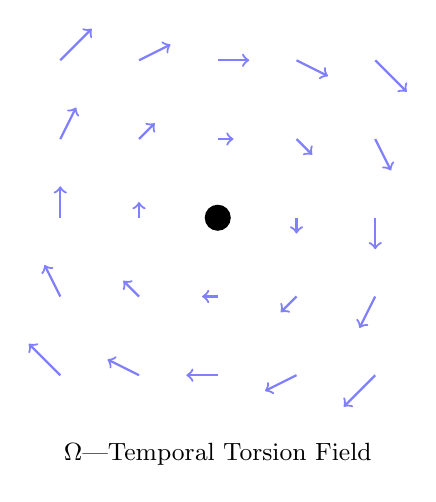
\begin{tikzpicture}[
    vec/.style={->, thick, draw=blue!50}
]

\foreach \x in {-2,-1,0,1,2}{
  \foreach \y in {-2,-1,0,1,2}{
     \draw[vec] (\x,\y) -- ++(0.2*\y,-0.2*\x);
  }
}

\node[circle,fill=black,minimum size=7pt] at (0,0) {};

\node at (0,-3) {\small $\Omega$---Temporal Torsion Field};

\end{tikzpicture}